\documentclass[a4paper,12pt,twoside]{article}



\title{Narrative Visualisation Project: NBA athletes are getting taller and heavier}

\author{Tung X. Nguyen}
\date{\today}

\setcounter{tocdepth}{3}


\usepackage{tikz,pgfplots}

\pgfplotsset{compat=1.10}
\usepgfplotslibrary{fillbetween}
\usepackage{apacite}
\usepackage{bm}
\usepackage{url}
\usepackage{amsmath}
\usepackage{indentfirst}
\usepackage{amssymb}
\usepackage[showframe=false]{geometry}
\usepackage{booktabs}
\usepackage{amsmath}
\usepackage{tabularx}
\usepackage{systeme}

\usepackage{graphicx}
\graphicspath{ {./img/} }

\usepackage[english]{babel}
\usepackage[utf8]{inputenc}
\usepackage{fancyhdr}
\usepackage{listings}
\lstset{frame=tb,
  language=Bash,
  aboveskip=3mm,
  belowskip=3mm,
  showstringspaces=false,
  columns=flexible,
  basicstyle={\small\ttfamily},
  numbers=none,
  numberstyle=\tiny\color{gray},
  keywordstyle=\color{blue},
  commentstyle=\color{dkgreen},
  breaklines=true,
  breakatwhitespace=true,
  tabsize=3
}

\setlength{\headheight}{15.2pt} 
 
\pagestyle{fancy}
\fancyhf{}
\fancyhead[LE,RO]{Tung X. Nguyen}
\fancyhead[RE,LO]{Narrative Visualisation Project}
\fancyfoot[LE,RO]{\thepage}
\fancyfoot[CE,CO]{\leftmark}

\renewcommand{\headrulewidth}{2pt}
\renewcommand{\footrulewidth}{1pt}
\numberwithin{equation}{section}



\begin{document}
\maketitle
ID: 30555418

Lab: 31

Tutor:  	Nicholas Spyrison
\thispagestyle{empty}

\tableofcontents
\listoffigures
\thispagestyle{empty}


\oddsidemargin = 22pt
\evensidemargin = 22pt
\marginparsep = 10pt
\marginparwidth = 35pt


\section{Introduction}
Even though I am not a big fan of basketball, I must admid that seeing the giants playing sports is quite exciting. Sometimes I ask myself: was they always this big? Look at the pictures of NBA ballers in the past, all I see are tall but skinny man, black and white. So, I come up with a speculation that statistically, body physique of basketball players in the modern time must be more impressive than their predecessors as they get better nutrition and better coaches. My visualization is created in the purpose of testing this hypothesis, but it is also useful for exploration as well in case you want to see where your favorite player stands in the league in term of height and weight.

The next question I want to address via interactive visualization is how foreign players look like in comparison with the American players. The league is fiercefully competitive, and I doubt that talents alone are not enough for a foreign player to get the approval from picky NBA scouts. Therefore, I also want to compare the physique of this two group, in the hope of seeing some interesting disparities that are statistically significant.

Finally, for this narrative project, I want to show how the distribution of PER, which is a popular index of performance in NBA, varies between height ranges. It is interesting to find out that bigger is not always better in the NBA. Also, in the spirit of a team sport, I also want to see the performance of players in comparison with their teammates. It is true that for some team, only one or two individuals take all the glory while the rest is forgotten, and I am not in favor of this trend.

\section{Design}
\subsection{Thought process}
Even though I am not a professional in design, I tried my best to be logical in the design process. Firstly I ask myself how the final result looks like, what types of charts I want to show. After generating several ideas in the first of the five design sheets, I chose to stick with simple graphs including scatter plot, boxplot, density plot and histogram to elaborate in the next three sheets. Next, I find ways to customize these graphs, create more opportunity for interaction. It comes natural to me that I have to give users more option to filter the data they want to see on the chart. Then I ask myself: what options are to be given, and how I represent them in the app. After answering all of these questions, the layout becomes much clearer, and the remaining work is simply tuning size, colors until I am satisfied with what I see.


\subsection{Tuning ideas}
At first I think it is a good idea to do every thing in d3. After finishing the d3 assignment, I find it not too difficult to draw a chart in d3. However, I was not sure if I had enough time to learn how to add many filters into the visualization. Therfore, I chose to stick with shiny in the end as a safer option.

As stated above, I think of many possible options for interaction. Some interesting ideas include: A slider bar that indicate the range of Draft Year for the first app (Figure 1), colorize dot according to their nationality (for the first app) or their team (for the second app, Figure 2). For both app, I also thought of adding text label to the outliers (players with unique physique or outstanding PER score). These ideas are not bad, I included them in sheet 2 and 3. However, in the end, I found these visual components a little distracting and decided not to add them to my final product.
\begin{figure}[h]
\caption{Candidate idea: Draft Year slider bar}
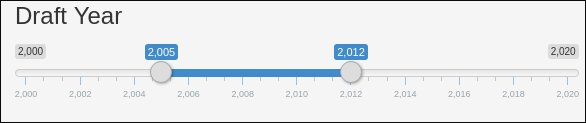
\includegraphics[scale=0.35]{op11.jpg}
\centering
\end{figure}
\begin{figure}[h]
\caption{Candidate idea: Colorize by team name}
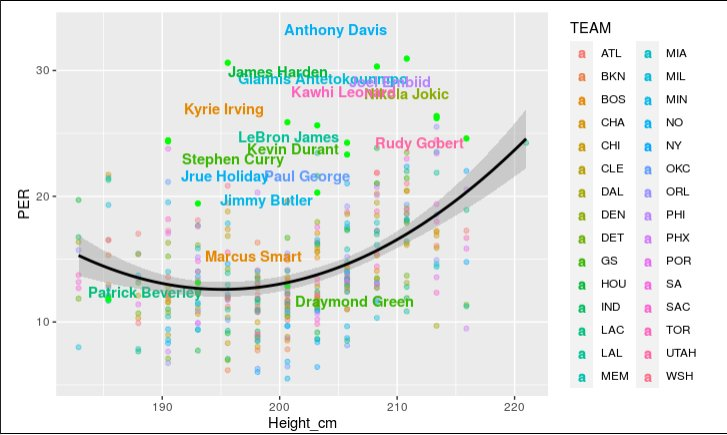
\includegraphics[scale=0.35]{op12.jpg}
\centering
\end{figure}


To make the most out of the visualization, I  decided to supplement the scatter plot with a small minor plot: density plot or boxplot. For the first app, both density plot and boxplot is good, but I chose density plots because I can overlap them for comparison. For the second app, boxplot proves to be better because sometimes the sample is too small, which is not suitable for density plot.
\begin{figure}[h]
\caption{Boxplot for the second app}
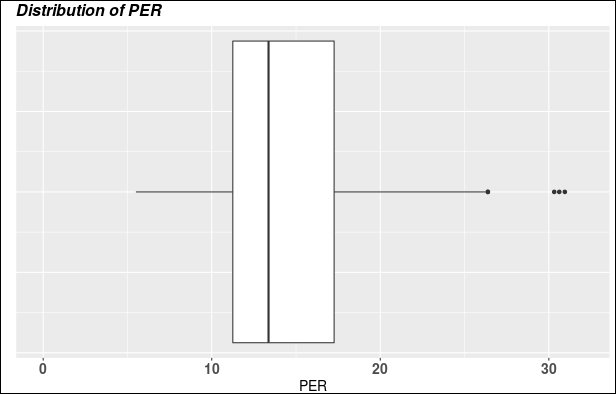
\includegraphics[scale=0.35]{box.jpg}
\centering
\end{figure}

\subsection{Final design}

The final designs are shown in Figure 4 (first app) and Figure 5,6 (second app) and in the design sheet 4 and 5 (see Appendix). For both of these apps, I believe that I cannot go wrong with simplicity and compactness. The visualization provides enough information and the clues of interaction are also very obvious, which means little to no time for training to use. Eventhough it is possible to add more options, I do not think that is necessary. Furthermore, I want to represent a coherent narrative with this visualization tool, and this final design do the job well as I see it.
\begin{figure}[h]
\caption{Height and Weight distribution and t-test}
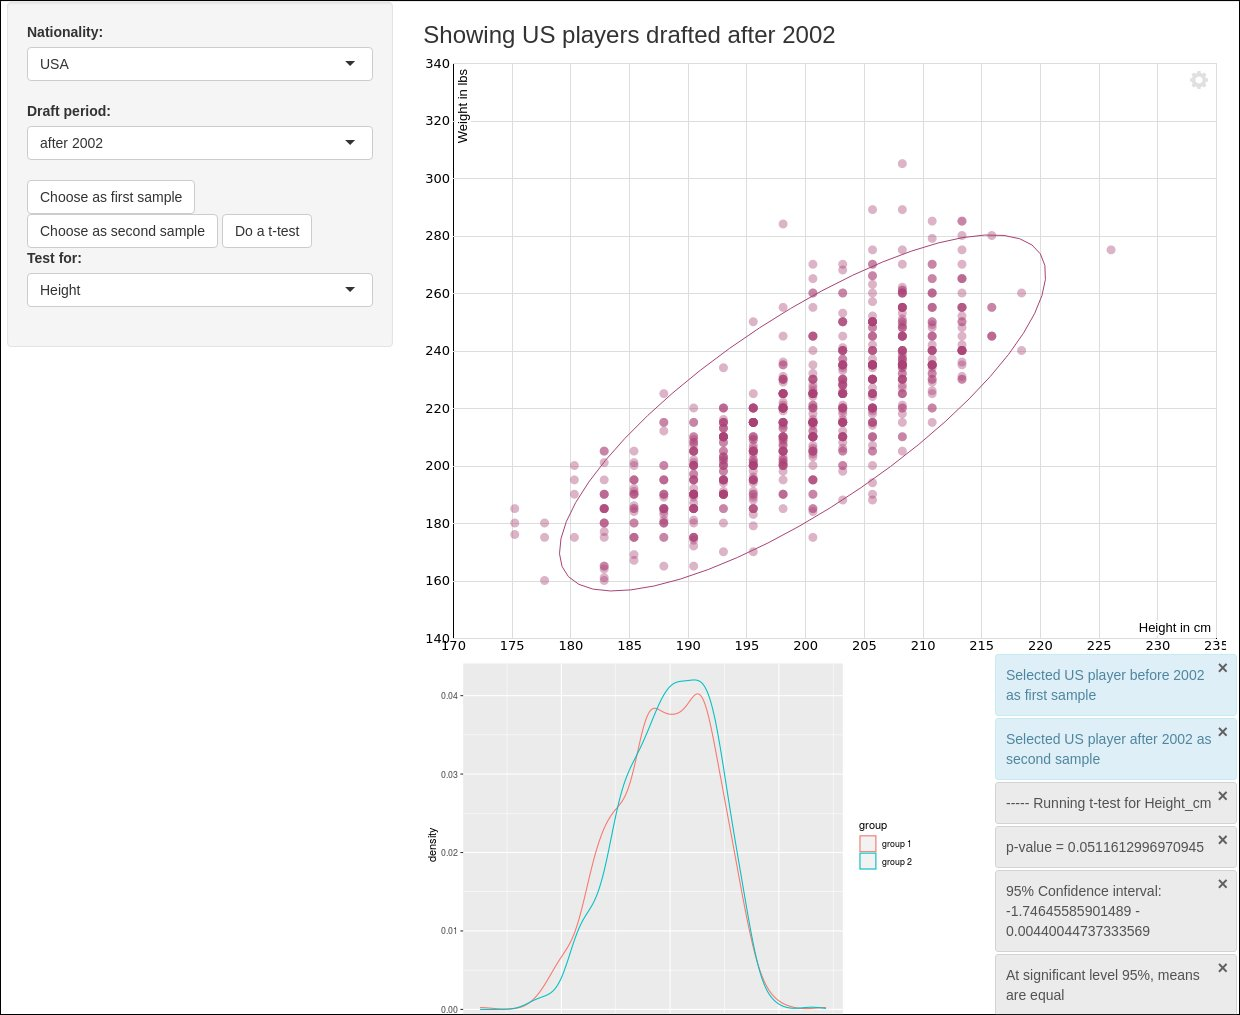
\includegraphics[scale=0.35]{op1.jpg}
\centering
\end{figure}
\begin{figure}[h]
\caption{PER and height for players in the same team}
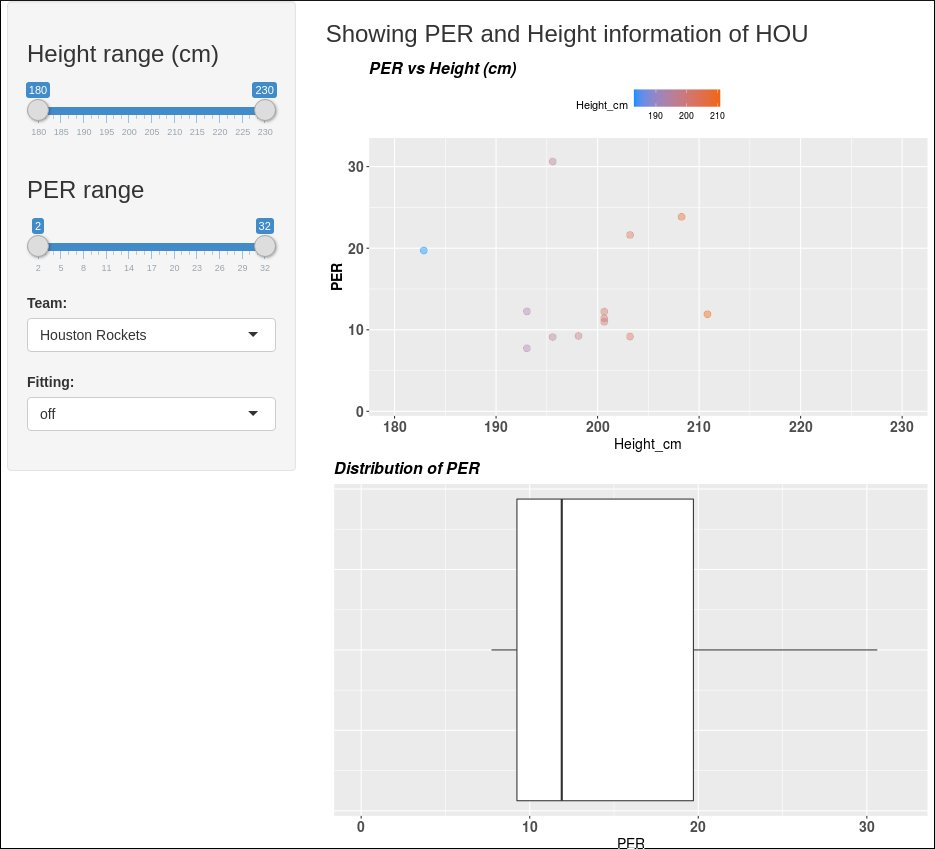
\includegraphics[scale=0.35]{op2.jpg}
\centering
\end{figure}
\begin{figure}[h]
\caption{PER and height for players in a height range}
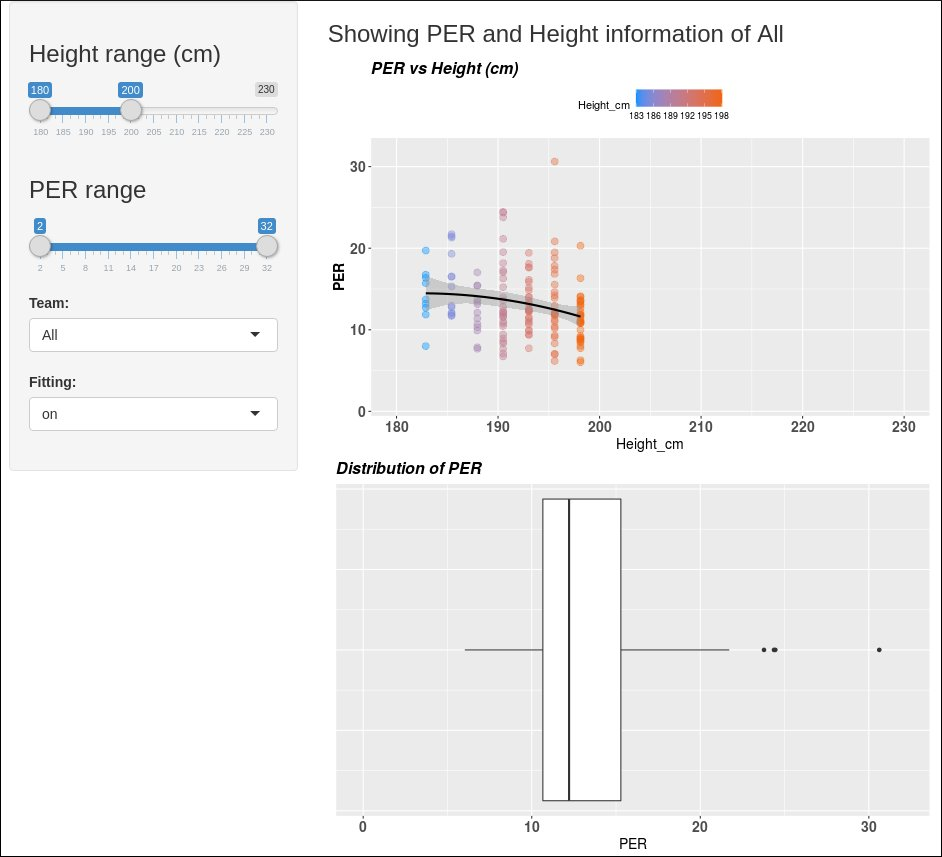
\includegraphics[scale=0.35]{op21.jpg}
\centering
\end{figure}


\section{Implementation}
\subsection{The distribution of Height and Weight}

For this visualization, I chose scatter plot because it is the most suitable for discoveries with 2 features. I used scatterD3 to draw the scatter plot instead of ggplot because it supports tooltips and zooming much better. The resulting scatter plot allows user to zoom in a point of a plot and highlight any point that is hovered on. The tooltip shows players' name, height in centimeters weight in pounds, and the country they are from. Other than that, when comparing two samples, I still used geom\_density in ggplot to draw overlayed density plots. 

The trickiest part in this visualization is to combine two vectors of different length into one single dataframe so that I can pass it to geom\_density, which I solved by a helper function I wrote myself (I could not find any available function that do the same thing, probably because it is not a popular problem). The helper function is simple but it does well what I expect it to do.


The result is satisfying: The visualization let the user pick any two groups based on draft period and nationality, visualize  them with scatter plot, then perform a t-test to compare the means of two group. The interaction is in the form of button, using actionButton and observeEvent objects in R, with clear and concise messages: "Select as sample 1", "Select as sample 2", "Do a t-test". Users can also choose which index to test for: height or weight. The consequence of any action is confirmed by notifications, which automatically fade away after a defined number of seconds. This interaction also guarantees that the user must pick two samples before conducting a test: a message will be displayed telling the user to pick the missing sample. Upon selection, each sample is assigned to a reactiveValues, and this is revolutionary at least for me. I can then manipulate these values as if they were global values and use them for the test and for the density plot. I also make sure that the result of the test is automatically intepretted (based on p-value) so that a user who do not know statistics well can still understand it. Combined with the overlayed density plot, I believe that my visualization is robust and somewhat scalable to other data.

This app also provide the user with some relaxing rules for selection: for each filter Nationality and Draft period, there is the "All" option which means the corresponding filter will not be applied. This allow users to answer question such as: Are US-players who was drafted before 2002 are the skinniest, by comparing this sample (as the first sample) with the whole dataset (as the second sample).


\subsection{PER and Height, Weight}

This app is my best attempt to show how PER varies across height range and across teammates as well. The data is collected from ESPN for the regular season 2018-2019. Firstly, users can filter the kind of players they are looking for using 2 slider bars that indicate PER range and Height range. An option is open for the fitting line if the user want to see the overall trend among a group of player. This visualization helps answer questions such as: as the height goes from 190 to 200cm, is the PER going upward or downward? This simply indicates whether a big guard is better than a small guard. To help users with navigation, the scale limit is fixed, keep the chart from rescaling after each interaction with the slider bars. A tooltip is also added to this app to show the players' name upon hovering.

Below the scatter plot is a boxplot that simply shows the distribution of the PER index. This simple tool helps reveal some interesting patterns: if the PER slider is set to full and the Height slider is set with a range of 10cm, upon moving this slider from left to right, the boxplot also moves as well, firstly to the left and then to the right. This may implie that under a certain height, bigger size correlates with decrease in performance.

Other than that, the user can play with the "Team" option to check the performance of players in a team. A short boxplot will indicate the consistency of a team, while a wide one with some outliers may tell the opposite story.

\section{User guide}
\subsection{The distribution of Height and Weight}

\subsubsection{Launching}
From the "final" directory, open the command line interface and launch the app:
\begin{lstlisting}
$ Rscript -e 'library(methods); shiny::runApp("dist_shinyapp/", launch.browser = TRUE)'
\end{lstlisting}
This will open the app in the default browser.
\subsubsection{Filtering}
Filter the target group with the "Nationality" tab and the "Draft period" tab. A reactive title is shown on top of the interface to confirm your selection. Observe and interact with the scatter plot: drag, zoom, hovering. The ellipse tells where most of the data is at. Discover the data points outside this ellipse (outliers) to see their detail. Try to find Yao Ming (China), Shaquile O'Neal and Zion Williamson (USA).
\subsubsection{T-test}
Capture the filtered group using the button "Choose as first sample". Filter another desired group and capture it with "Choose as second sample". A message will be displayed to confirm your selection.

Then, simply click the "Do a t-test" button. A density plot is instantly rendered right below the scatter plot, showing the distribution of the two group. The t-test will tell if the mean of the two group is significantly equal or not based on the p-value of t-test. If the confidence interval is positive, this means the first group has bigger mean and vice versa.
\subsubsection{Exit}
Simply go the the command line interface again and terminate the program. (Ctrl-C in Linux and Windows). Close the browser tab.

\subsection{PER and Height, Weight}
\subsubsection{Launching}
From the "final" directory, open the command line interface and launch the app:
\begin{lstlisting}
$ Rscript -e 'library(methods); shiny::runApp("per_shinyapp/", launch.browser = TRUE)'
\end{lstlisting}
This will open the app in the default browser.
\subsubsection{Filtering}
Filter the target group using 2 slider bars for "Height" and "PER" and the "Team" option. Turn on/off the fitting line with the "Fitting" option. The boxplot simply shows the information of the distribution of PER for the selected group.

Hover on any point to see the corresponding player' name.


\subsubsection{Exit}
Simply go the the command line interface again and terminate the program. (Ctrl-C in Linux and Windows). Close the browser tab.

\section{Conclusion}
\subsection{Findings Summarization}
\begin{itemize}
\item The mean height and weight of US NBA players are smaller than those of their foreign counterpart.
\item There is no significant differecnce between mean height and weight of US players drafted before and after 2002. The same is true for foreign players.

\item Under the height of 200cm, height and PER are not positively correlated. The opposite is true for height above 200cm.

\item Some coherent teams: Memphis Grizzlies, San Antonio Spurs, Charlotte Hornets, Dallas Maverick, Chicago Bull.
\end{itemize}
\subsection{Achievement}
\begin{itemize}
\item Two interactive shiny apps that can run with little errors.
\item A function that merge two vectors into a dataframe.
\item A t-test tool embedded in a shiny app that automatically interprets the output, also foolproof to a certain level.
\item tooltip embedded in scatterplot that shows extra information.
\end{itemize}
\subsection{New things I learnt}
\begin{itemize}
\item How to draw a scatter plot with simple tooltip in Shiny
\item How to create button and action in Shiny that unlocks another level of interaction.
\item How code is compiled in shiny. How to declare a reactive variable that acts as a global variable.
\item How to use 5 design sheets to plan the visualization.
\item Good visualization takes great time and attention to detail. I am sure that my product has a lot to be improved. If I have more time to finish it, I may try to position every component in a more harmonic layout.
\end{itemize}

\section{Appendix}

This section provides five design sheets.
\begin{figure}[h]
\caption{Sheet 1}
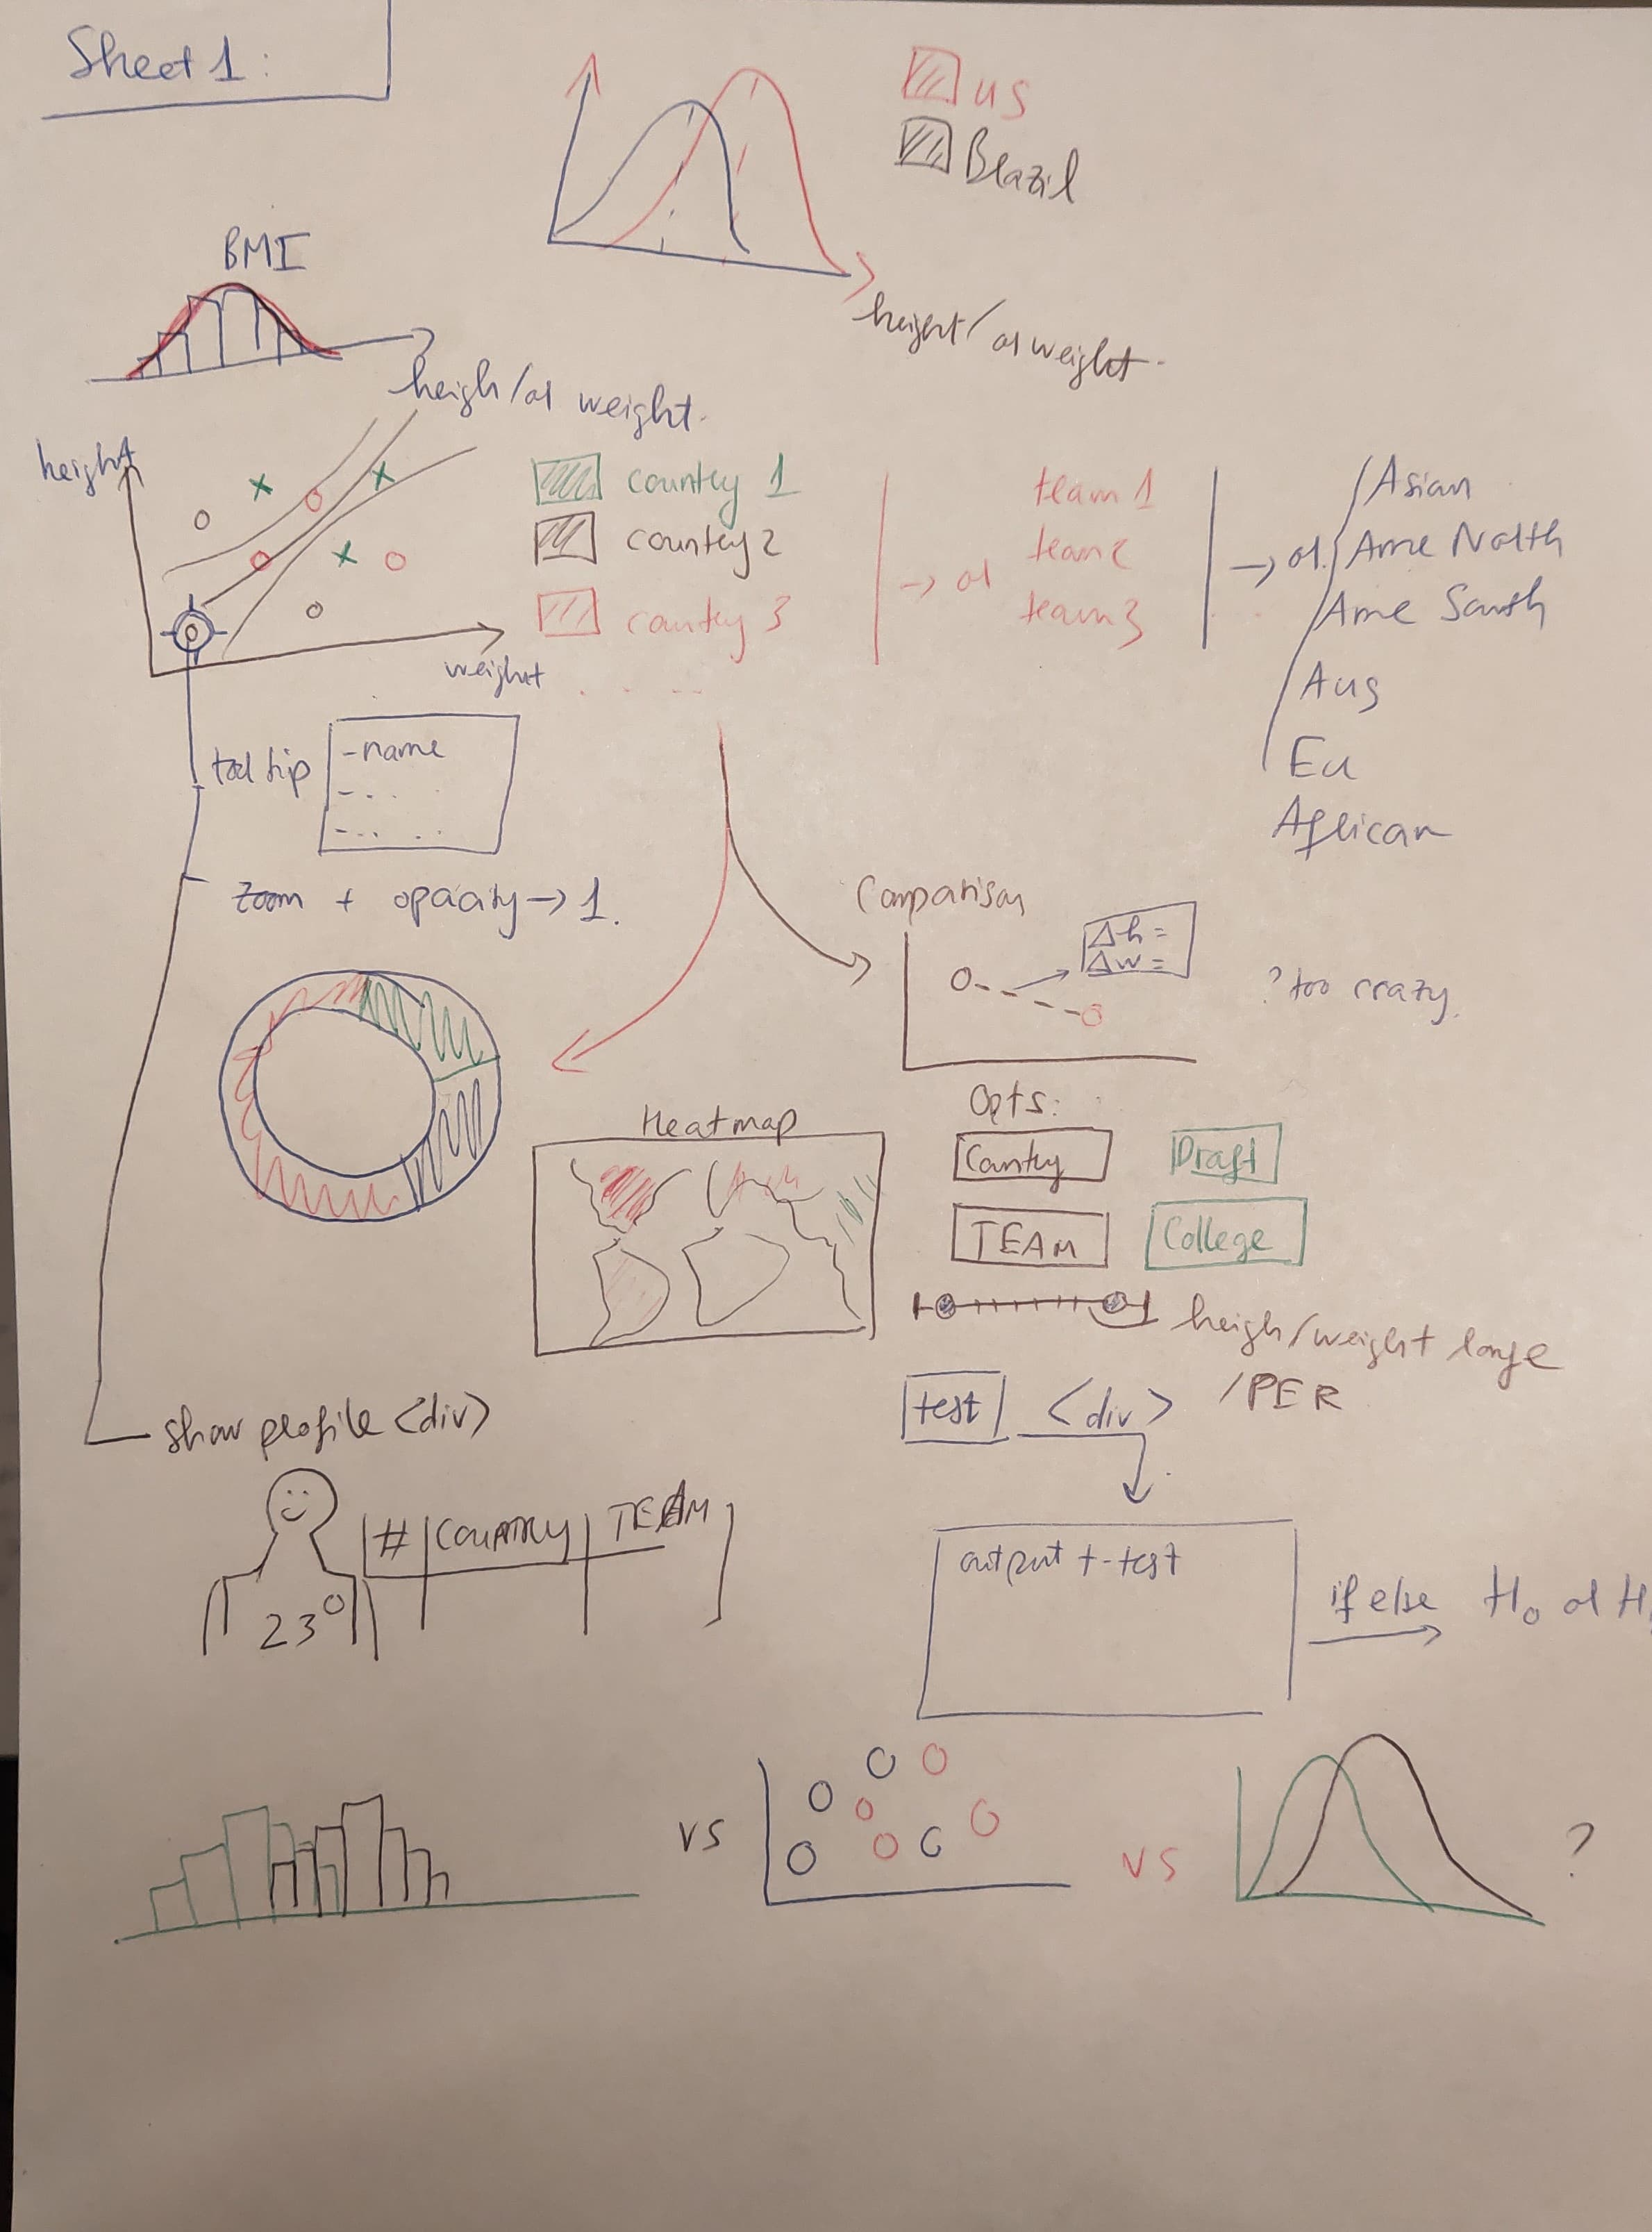
\includegraphics[scale=0.15]{o1.jpg}
\centering
\end{figure}

\begin{figure}[h]
\caption{Sheet 2}
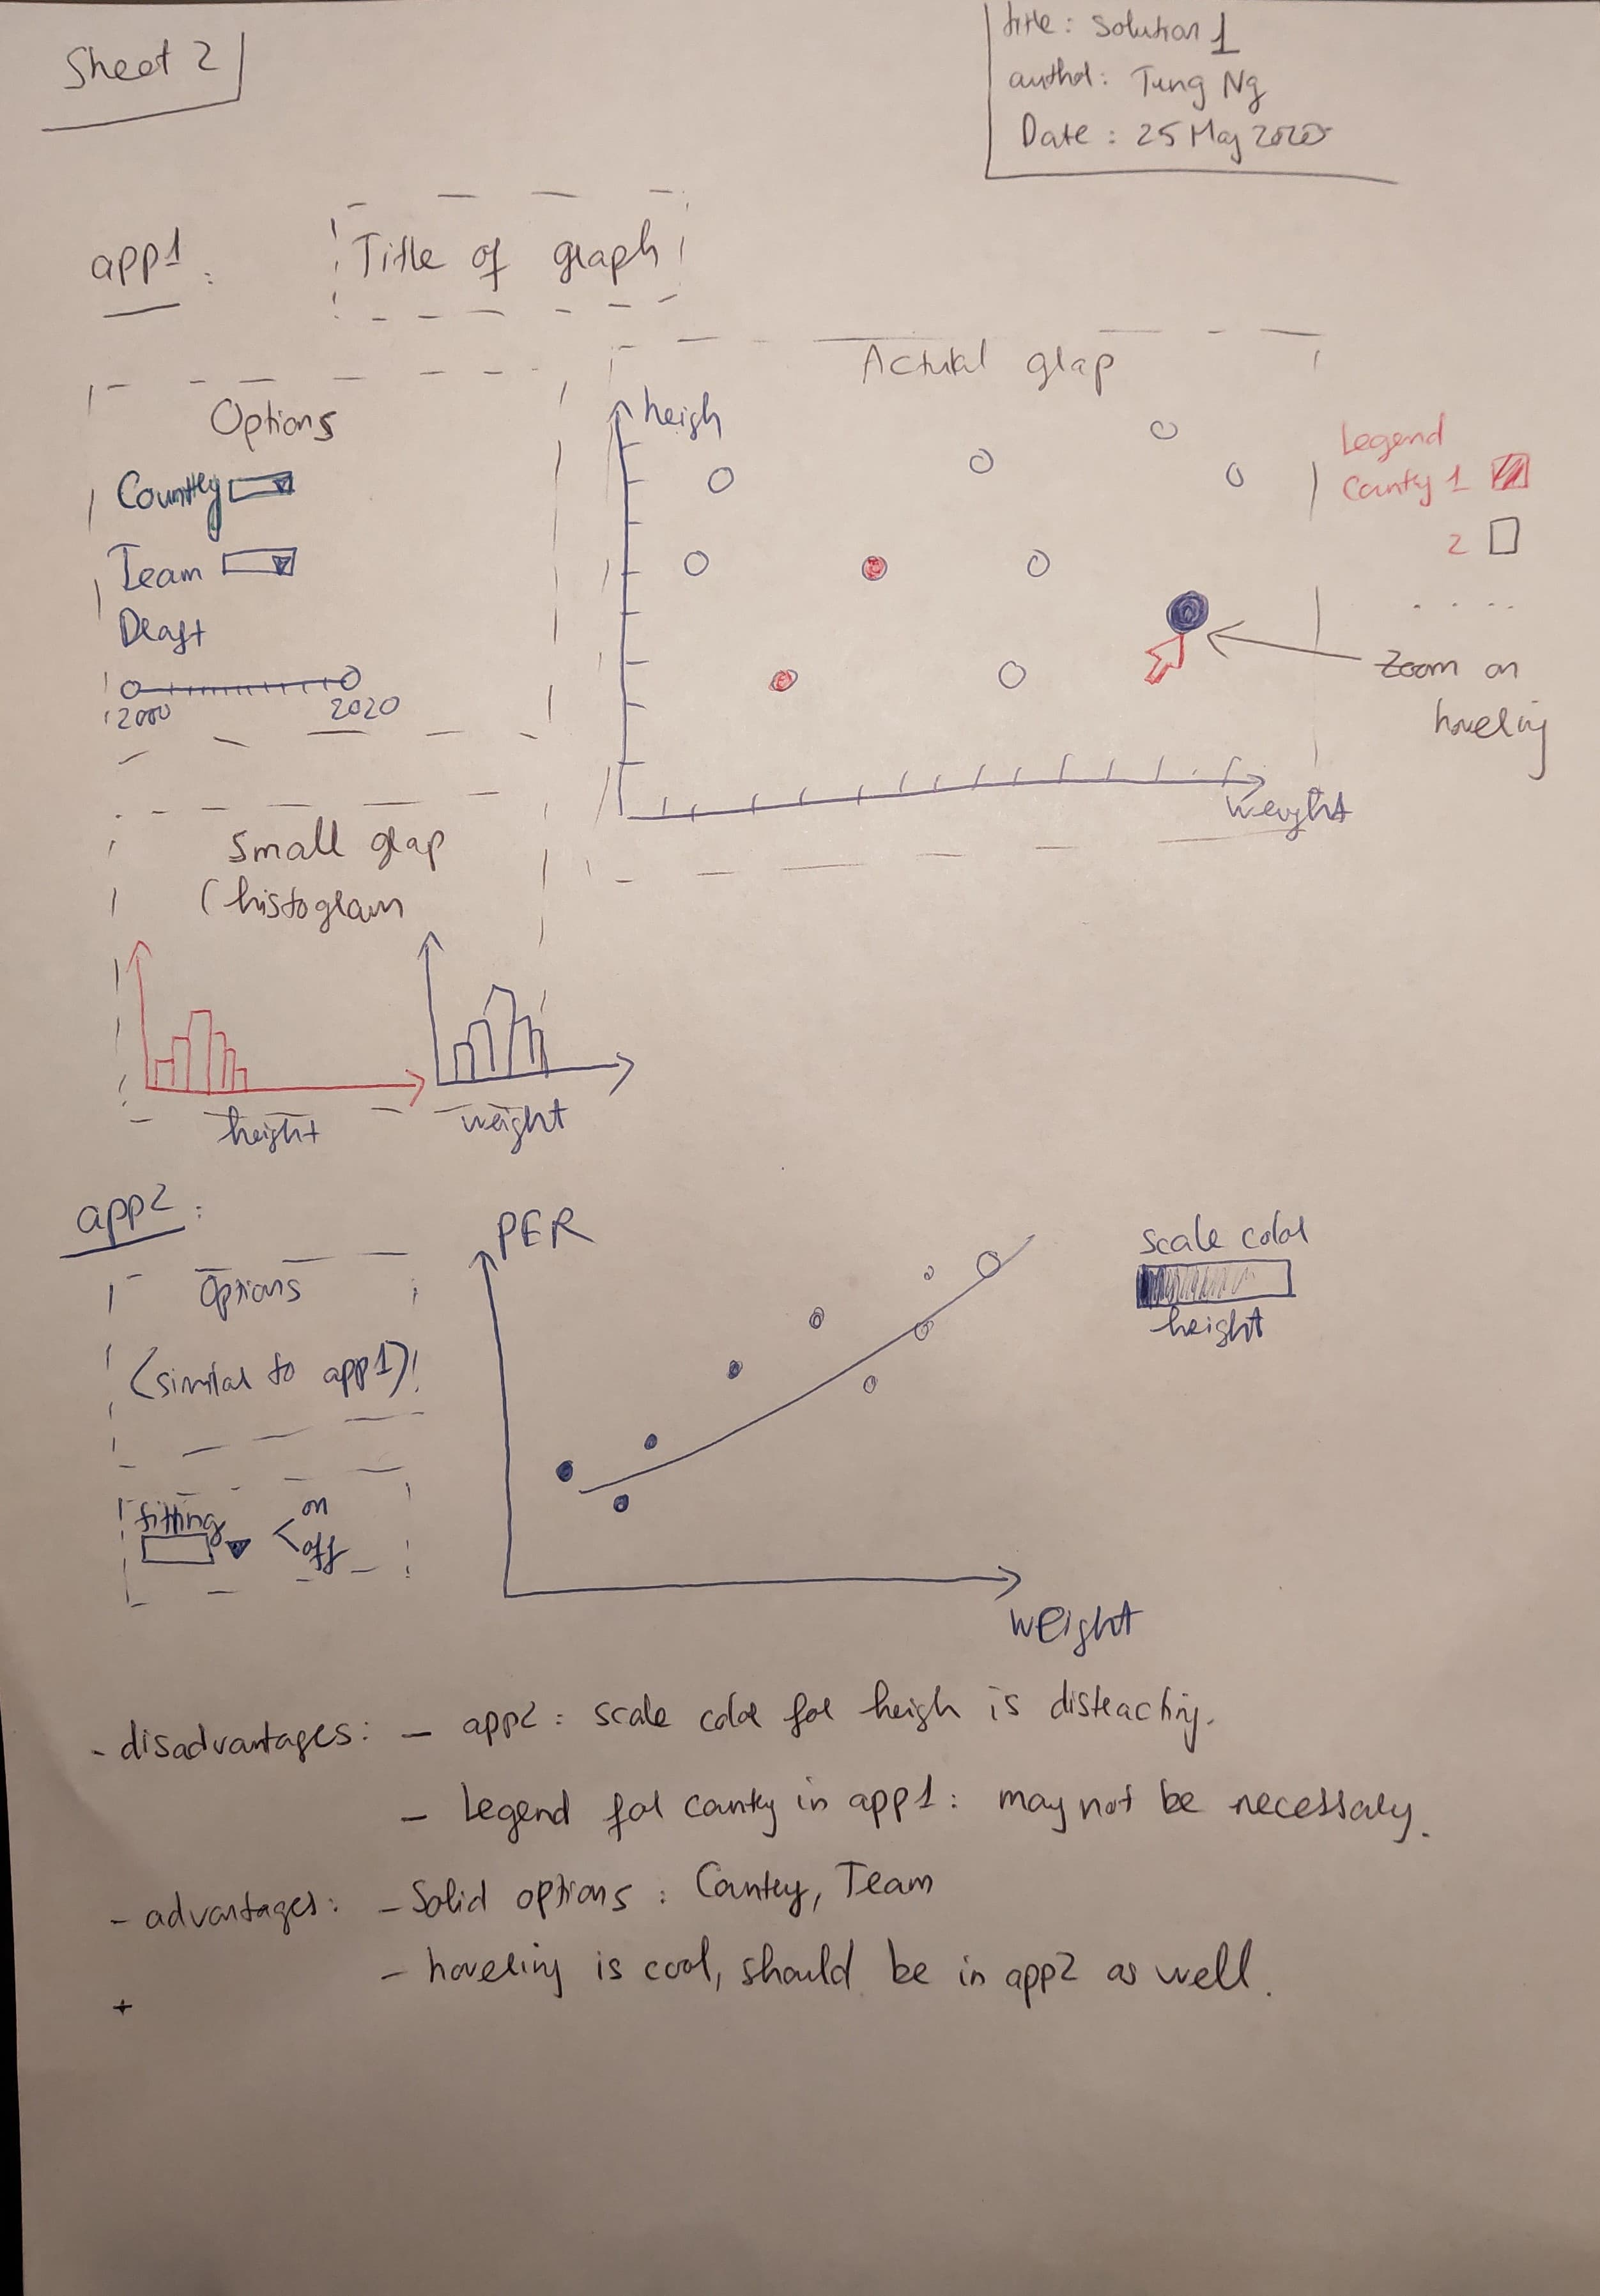
\includegraphics[scale=0.15]{o5.jpg}
\centering
\end{figure}

\begin{figure}[h]
\caption{Sheet 3}
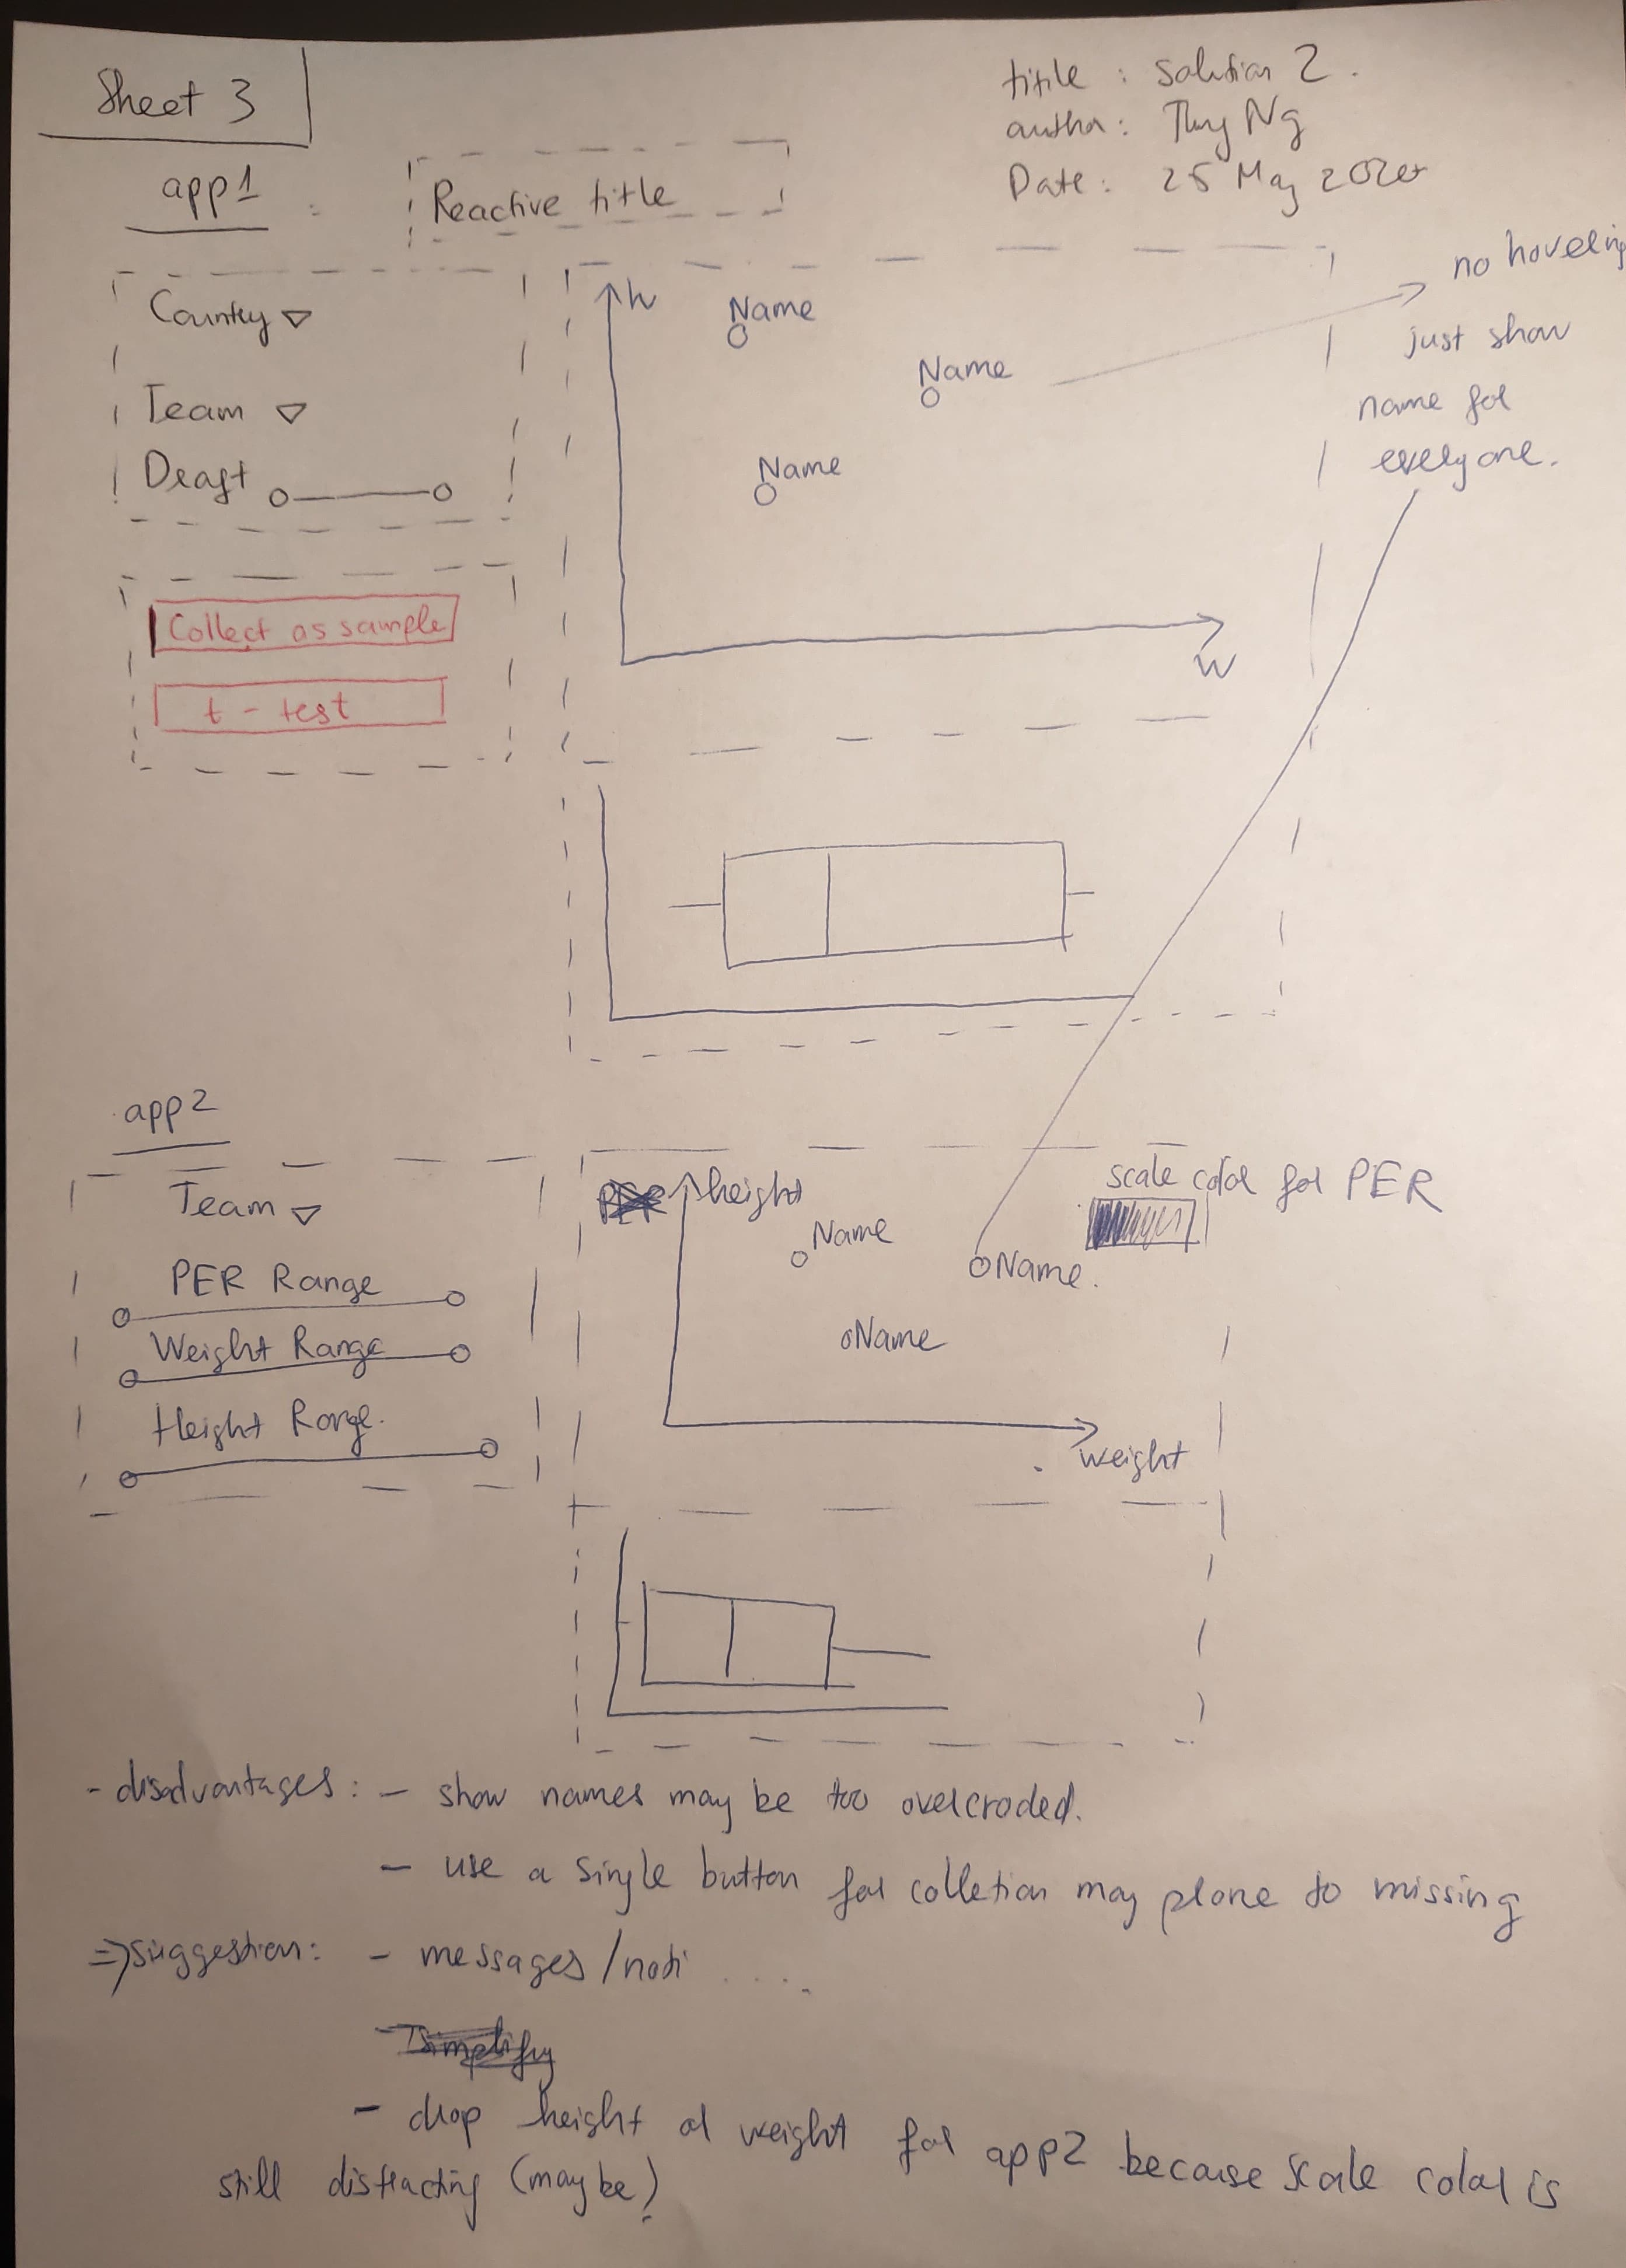
\includegraphics[scale=0.15]{o3.jpg}
\centering
\end{figure}

\begin{figure}[h]
\caption{Sheet 4}
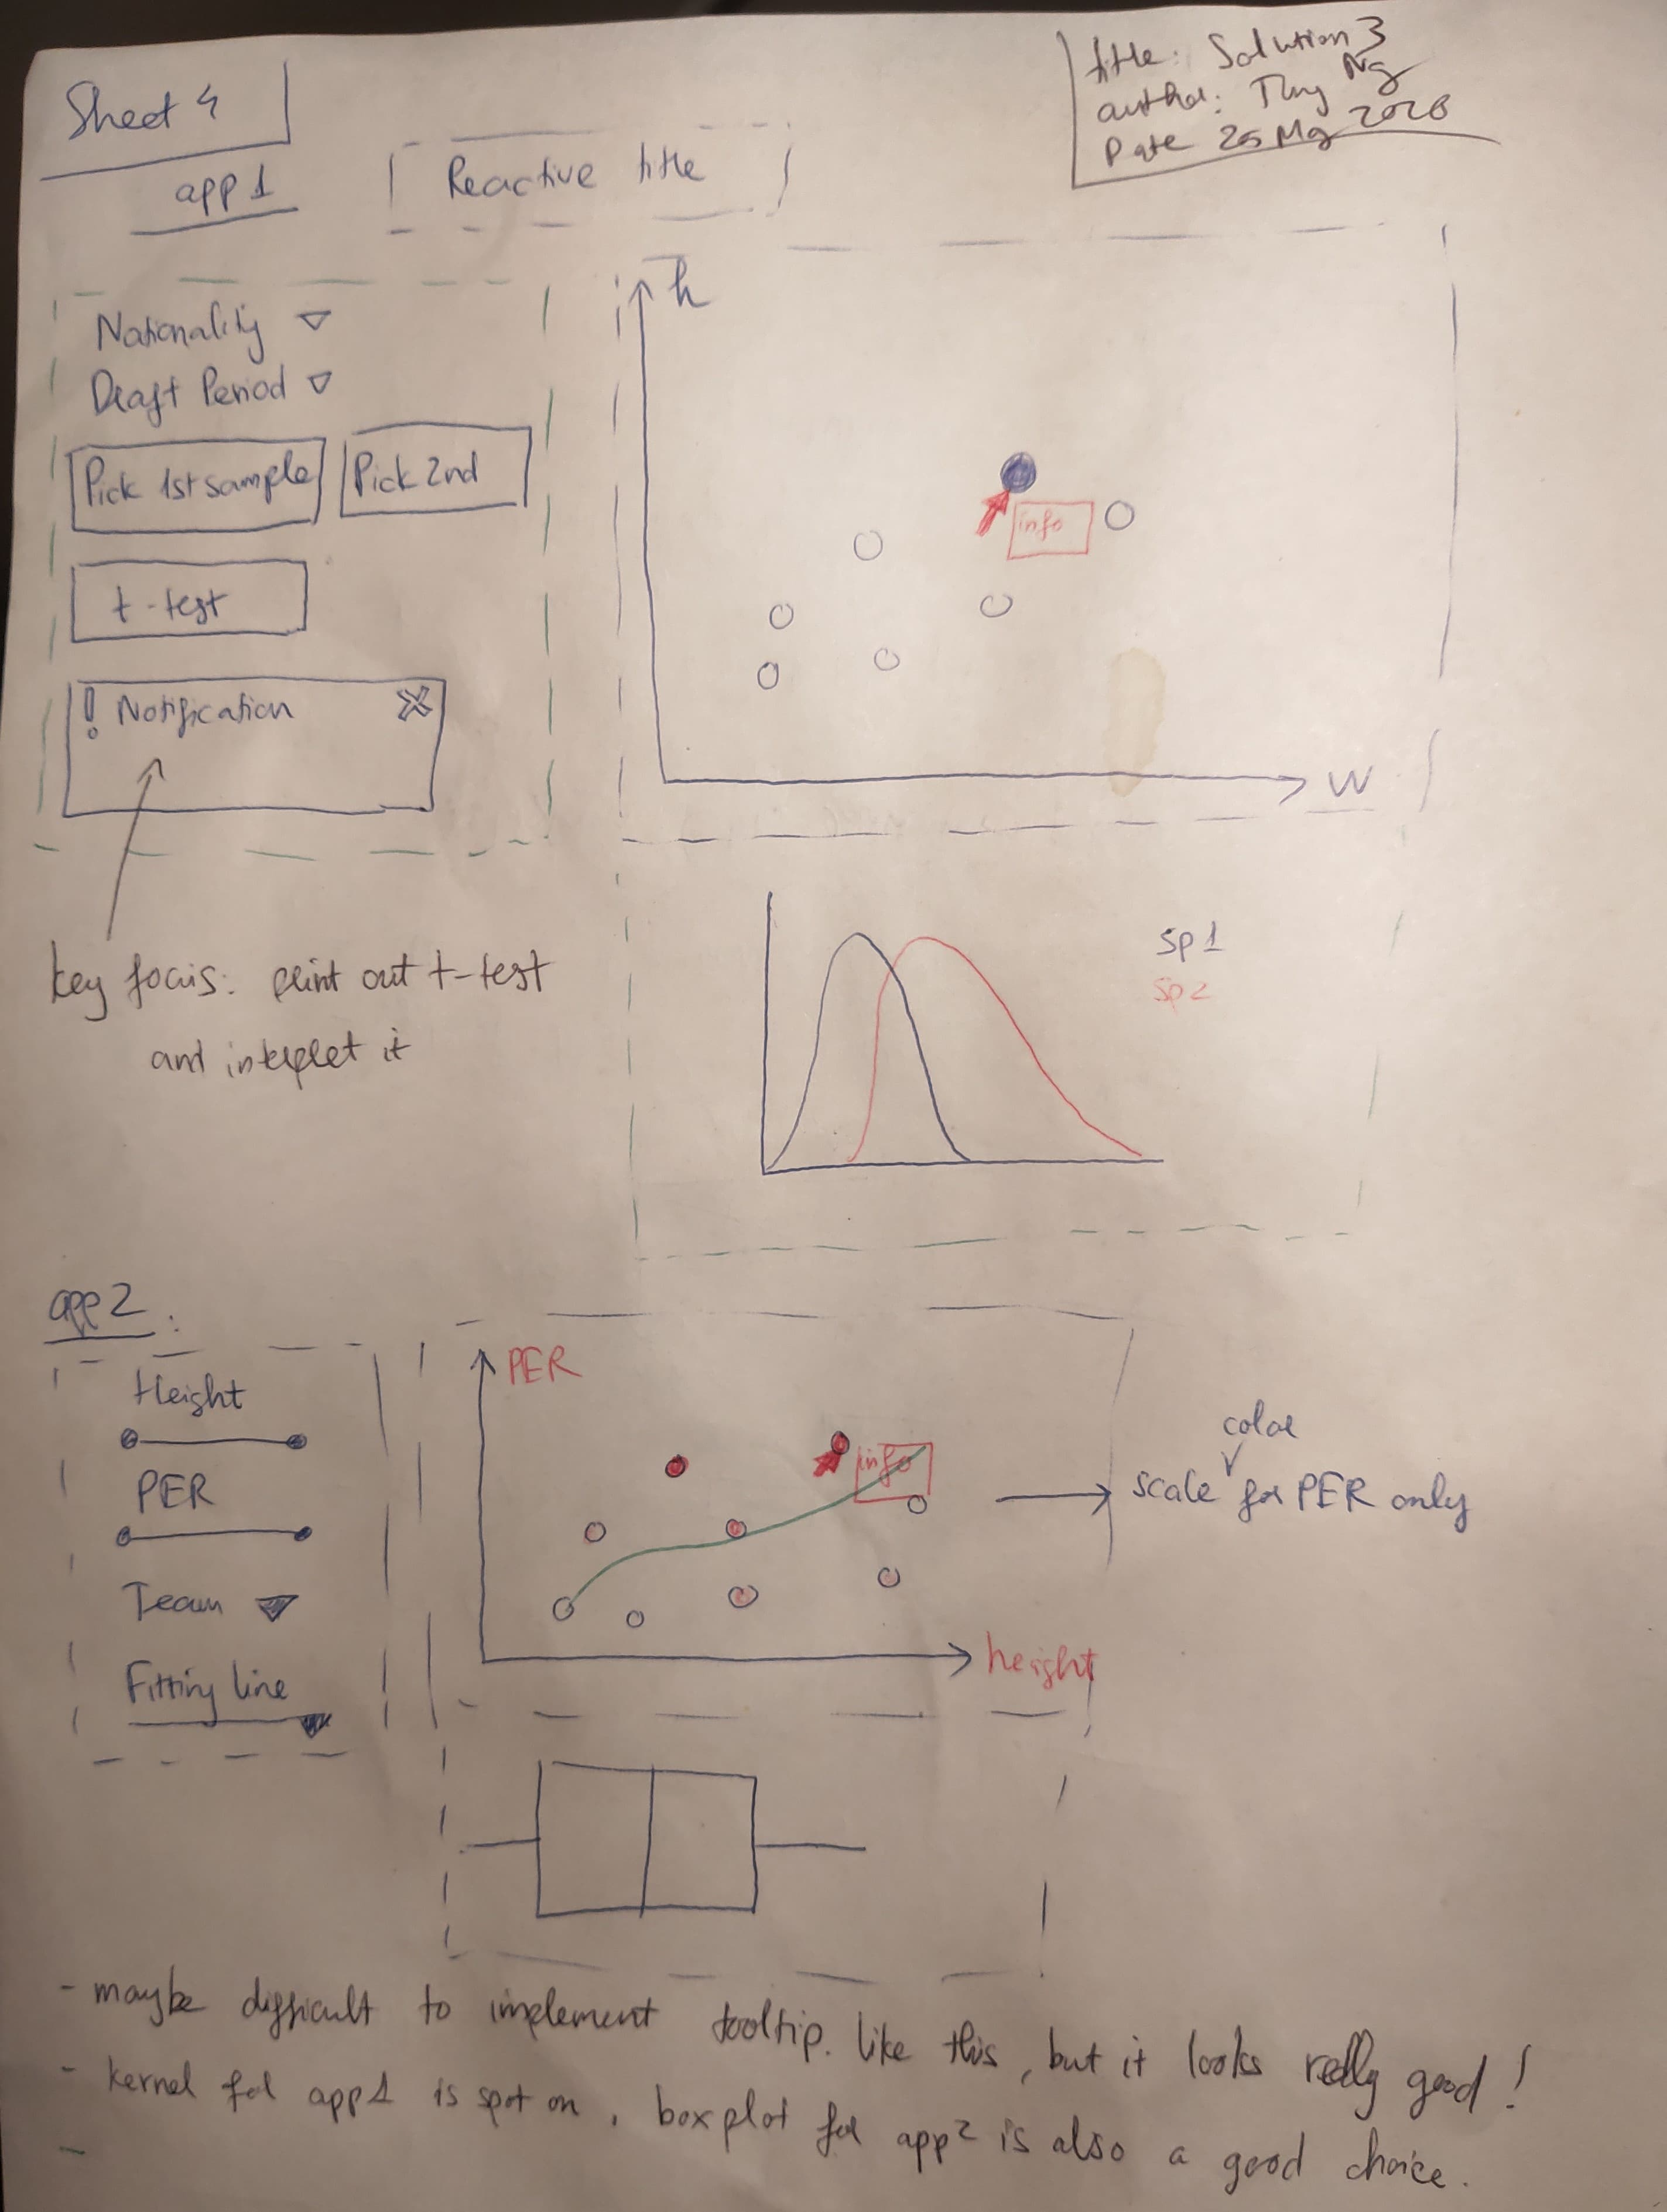
\includegraphics[scale=0.15]{o4.jpg}
\centering
\end{figure}

\begin{figure}[h]
\caption{Sheet 5}
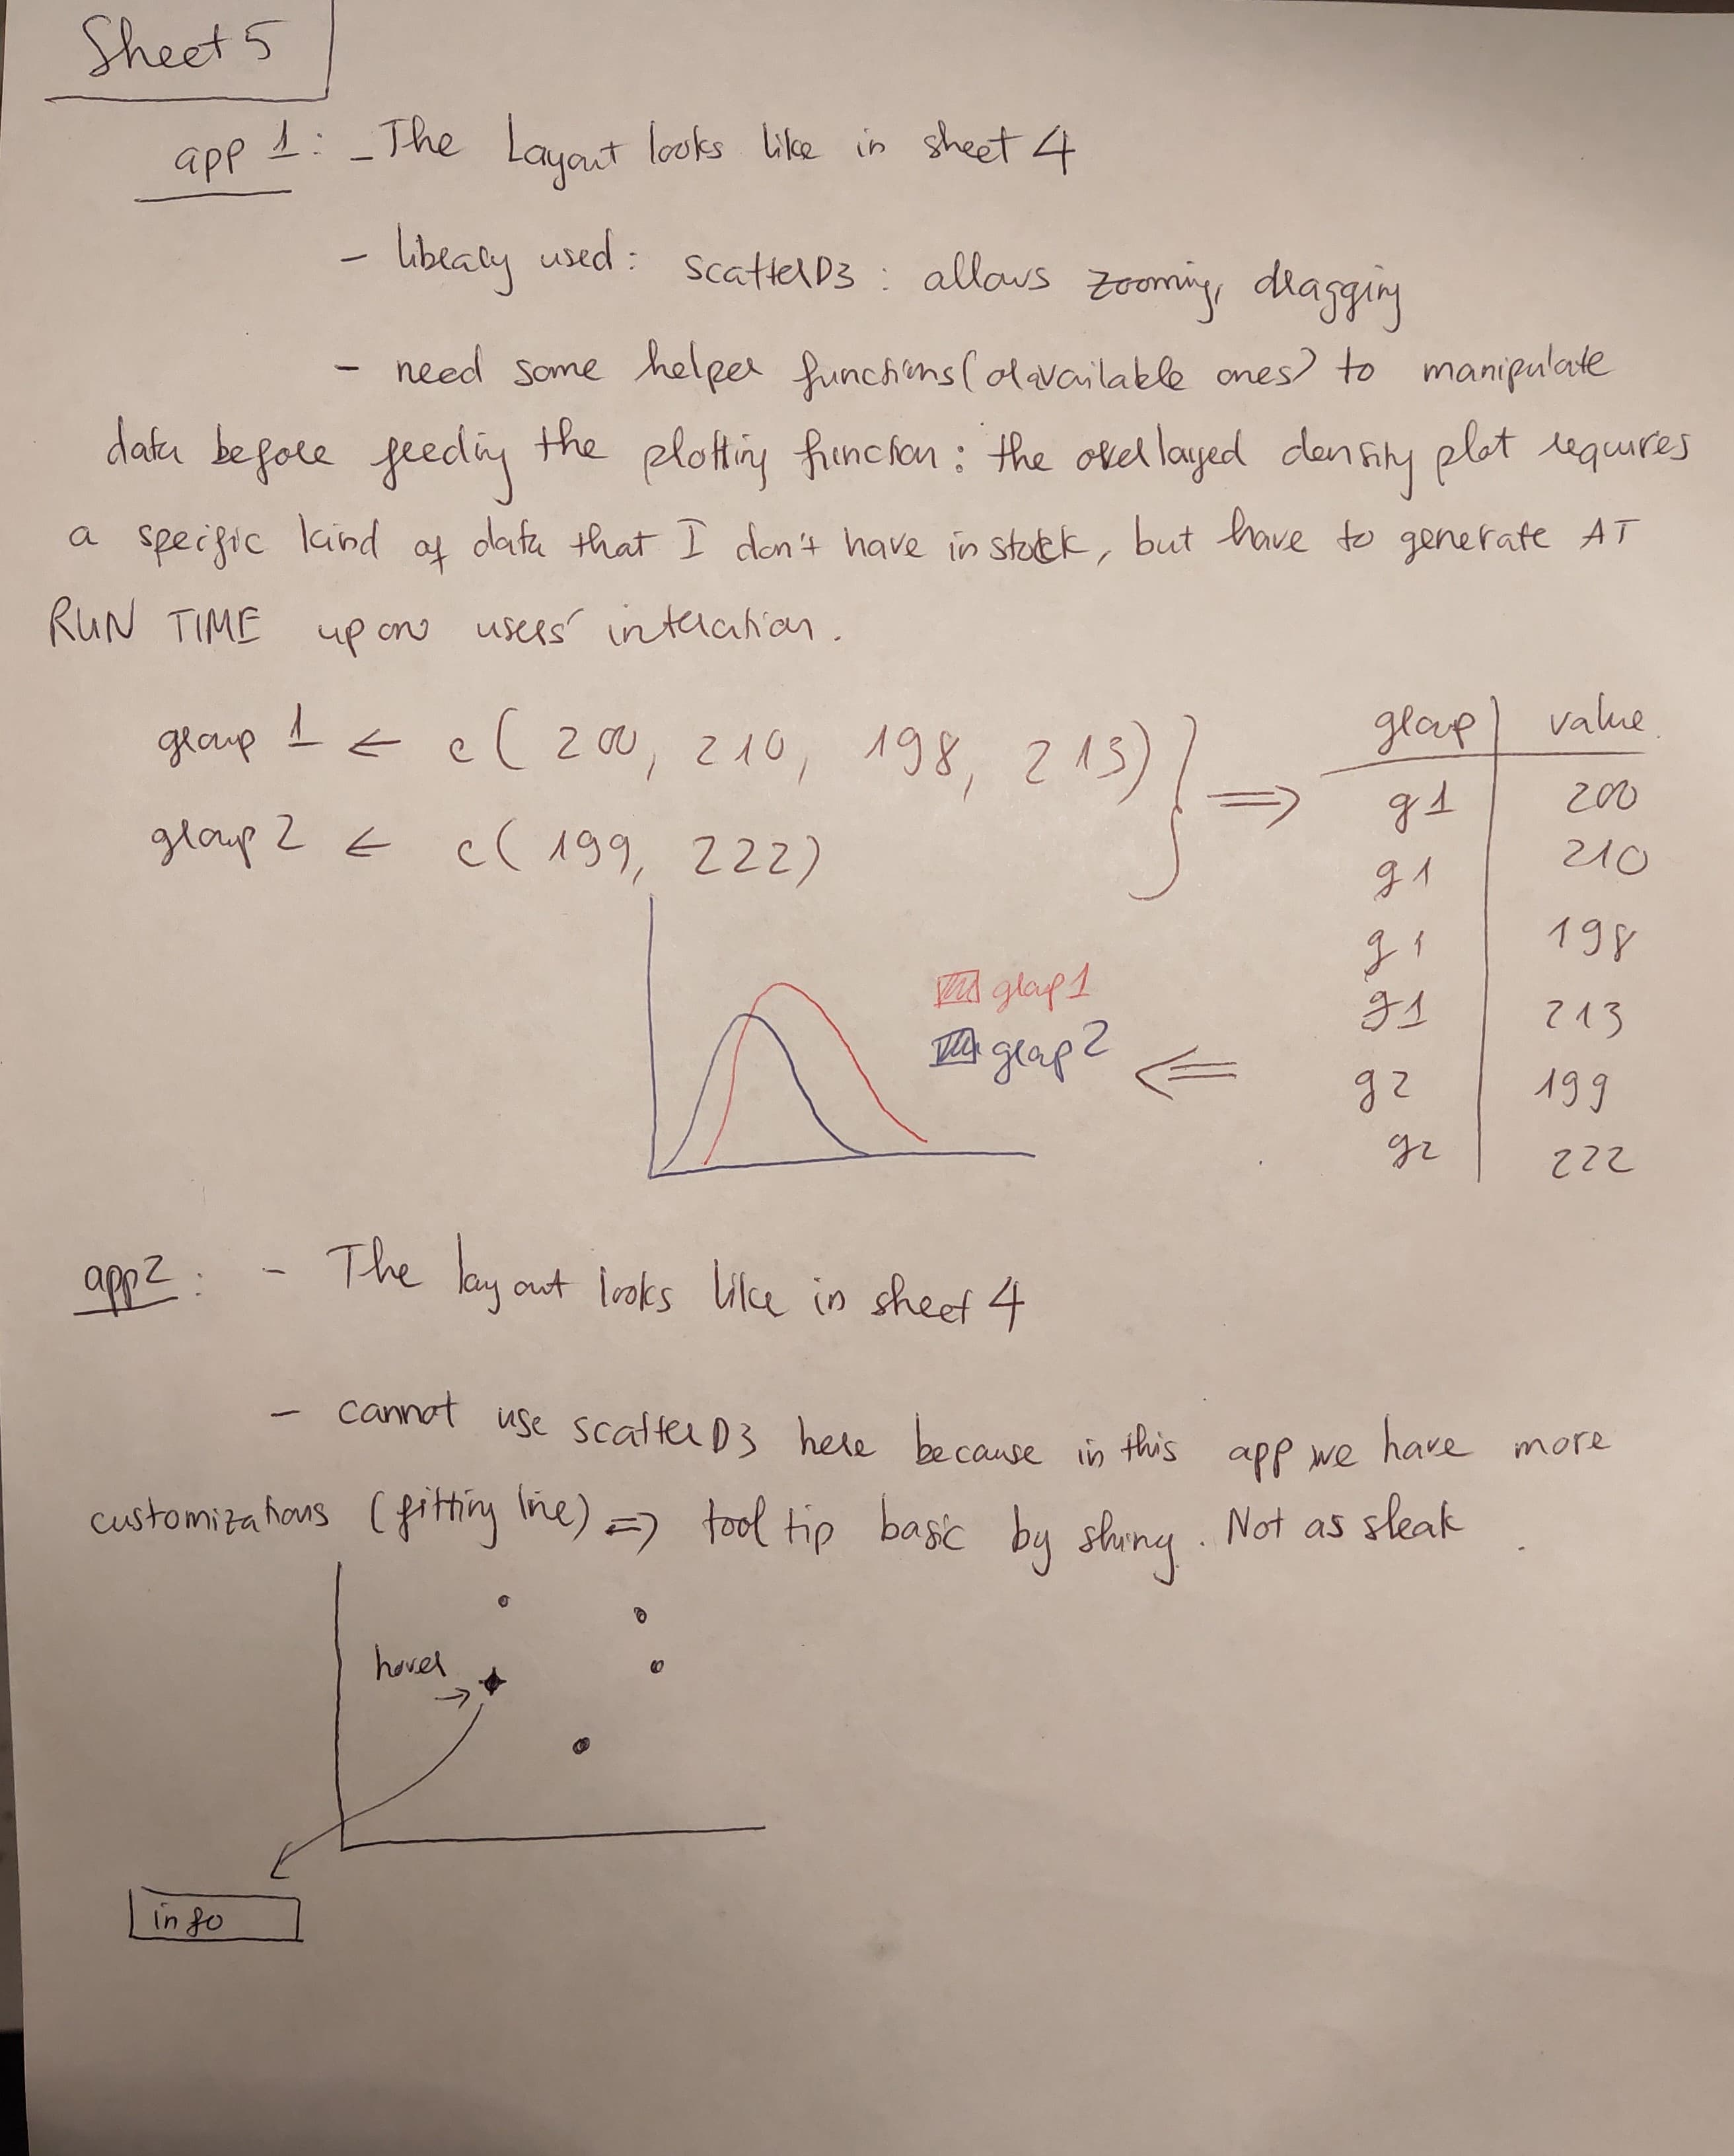
\includegraphics[scale=0.15]{o2.jpg}
\centering
\end{figure}
\end{document}
